\documentclass[]{IEEEtran}
%\IEEEoverridecommandlockouts
% The preceding line is only needed to identify funding in the first footnote. If that is unneeded, please comment it out.
\usepackage{cite}

% Your packages go here
\usepackage[utf8]{inputenc}
\usepackage{romannum}
\usepackage{graphicx}
\usepackage{caption,subcaption}
\usepackage{listings}
\usepackage{color}
\usepackage{url}

\definecolor{dkgreen}{rgb}{0,0.6,0}
\definecolor{gray}{rgb}{0.5,0.5,0.5}
\definecolor{mauve}{rgb}{0.58,0,0.82}

\lstset{frame=tb,
  language=python,
  aboveskip=3mm,
  belowskip=3mm,
  showstringspaces=false,
  columns=flexible,
  basicstyle={\small\ttfamily},
  numbers=none,
  numberstyle=\tiny\color{gray},
  keywordstyle=\color{blue},
  commentstyle=\color{dkgreen},
  stringstyle=\color{mauve},
  breaklines=true,
  breakatwhitespace=true,
  tabsize=3,
  literate={á}{{\'a}}1
           {ç}{{\c{c}}}1
           {ü}{{\"u}}1
           {é}{{\'e}}1
}

\def\BibTeX{{\rm B\kern-.05em{\sc i\kern-.025em b}\kern-.08em
    T\kern-.1667em\lower.7ex\hbox{E}\kern-.125emX}}

\markboth{MC949/MO446 Computer Vision - HW1}{}

\begin{document}
  \title{Cartoonizing images with convolutions}
  \author{Darley Barreto, Edgar Tanaka, Tiago Barros
    \thanks{228120, 023577, 093125}
  }
  \maketitle
  
  \begin{abstract}
%     In this work, we use a mathematical operation called convolution, which applies a transformation in an image resulting in another image. With this operation, we are able to apply an infinite combination of kernels/filters to create new images. We combine kernels to create a cartoonized version of images, we divide this process into several small tasks, and in each of these, we show our results and compare with other approaches, and in the end, we show the resulting cartoonized images.


    In this work, we use image processing techniques such as filters, edge detection and color quantization in order to
    create a cartoonized effect on regular photograph images.
    As convolutions are key to both filtering images and finding edges, we explore a number of different kernels
    while showing our results in comparison with other approaches.
    At the end, we display the best cartoonized images produced by our experiments.
  \end{abstract}
  
  \section{Introduction}
  Image processing in the spatial domain is a visually rich area of study dealing with pixel-manipulation techniques.
  Images are treated simply as arrays of two or more dimensions.
  Normally, the matrix-based operations are performed between a larger matrix, representing the complete image,
  and a smaller matrix, which is known as a kernel. The kernel size and the associated values determine the
  impact exerted by it on the image considered.
  
  We first start by defining and implementing the convolution operation,
  then comparing it with the default implementation of OpenCV.
  As we want to perform convolution to cartoonize images, this process can be split into several small tasks
  such as:
  (\Romannum{1}) reducing colors/textures, since cartoons contain a smaller quantity of colors than real-world images,
  (\Romannum{2}) detecting edges is necessary to draw contour lines in the objects of the image,
  (\Romannum{3}) drawing lines, because cartoons have borders to separate colors and textures between objects.

  \section{Convolution}
  In its most general form, convolution $s(t)$ is an operation on two functions of a real-valued argument\cite{b1}
  $$
  s(t) = (x \ast w)(t)
  $$
  
  The first argument, $x$, to the convolution is often referred to as the input and the second argument, the function $w$, as the kernel. The output is sometimes referred to as the feature map.
  In terms of image processing, each convolution operation has a kernel which could be any matrix smaller than the original image in height and width. Each kernel is used for a specific task, such as sharpening, blurring, edge detection, and more.
  To do a convolution in an image using a kernel, we have to flip and ``slide'' the kernel on top of the image: for each pixel in the image, we position the kernel on ``top'' of it, so the middle element of the kernel is aligned with that pixel, then we multiply each element of the kernel with its corresponding element of the image matrix (the one which is overlapped with it), then we perform a summation of all product outputs and place the result at the same position in the output matrix as the center of the kernel in the image matrix\cite{b2}. 
  
  As an image might have any size, and so does the kernel, that is, the size of the image might not be multiple of the size of the kernel, thus a naive multiplication of the kernel by slices of the original image might not be possible. So we need to change the strategy of dealing with the borders, we choose to augment it in order to have an image proportional to the size of any kernel. We choose to augment the image by adding rows and columns full of zeros, which is called zero padding. Although there are other types of padding, such as constant, replicate, repeat, mirror, extend\cite{b3}, we choose to use zero padding because we think it is more reliable with the data matrix, that is, we are using data from the original image only, once the borders have not a constant values other than $0$ nor mirrored pixels.
  
  We implemented our own convolution operation, which runs in $\Theta(mnk^2)$, where $m$ is the width, $n$ the height and $k$ the kernel size. We ran four tests using different images and kernels for each one of them. Nevertheless, we ran the same tests using the convolution implemented in Python 3.7.0b3 OpenCV and the results are in the table below:
      
    \begin{table}[h]
    \centering
        \begin{tabular}{|c c c c c|} 
        \hline
            Experiment & Kernel size & Ours & OpenCV & Task\\ 
            \hline\hline
            1 & 3 & 13.9 & 0.015 & Sharpening\\ 
            \hline
            2 & 3 & 2.6 & 0.0033 & Embossing\\
            \hline
            3 & 5 & 7.7 & 0.0174 & Unsharpening\\
            \hline
            4 & 7 & 5.4 & 0.0105 & Gaussian blurring\\
        \hline
        \end{tabular}
        \vspace{1pt}
        \caption{Comparison of convolution tests running time (seconds).}
        \label{table:1}
        \vspace{-5pt}
    \end{table}
    
    The results of the four experiments show us that our implementation runs slower than the one in OpenCV. This is mainly because OpenCV uses optimized implementations such as Fast Fourier Transform (FFT), which lets us perform large-kernel convolutions in time that is independent of the kernel's size\cite{b3}. Also, it is written in C/C++, then when we install on Python, the library is downloaded, compiled and it is called by the Python interpreter as a binary or $.so$ (shared object) file, which is significantly faster than a Python implementation. Even though we use Numpy, the library is loaded into the main memory, which causes overhead and we do two plain Python \textbf{for} loops to perform the convolution on the image.
    
    Figure \ref{figure:conv} shows examples of performing convolution operations in two different images using our implementation and OpenCV's.
    
    \begin{figure*}[t]
      \centering
      \begin{tabular}{c c c}
      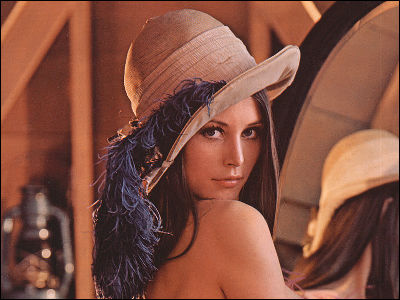
\includegraphics[width=0.23\linewidth]{./figures/2/lena.jpg} &
      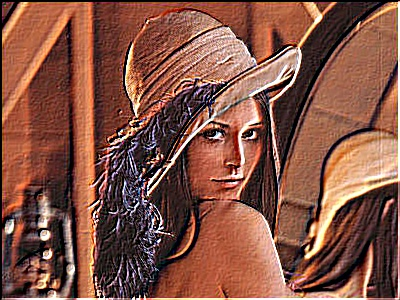
\includegraphics[width=0.23\linewidth]{./figures/2/lena-2-2.jpg} &
      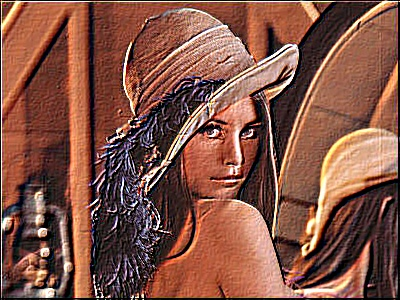
\includegraphics[width=0.23\linewidth]{./figures/2/lena-2-2-cv.jpg} \\
      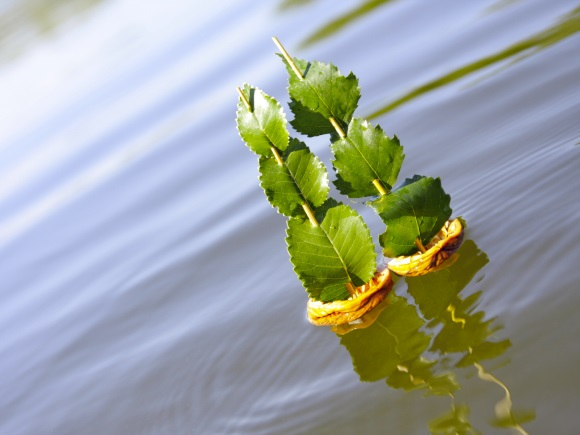
\includegraphics[width=0.23\linewidth]{./figures/2/lake.jpg} &
      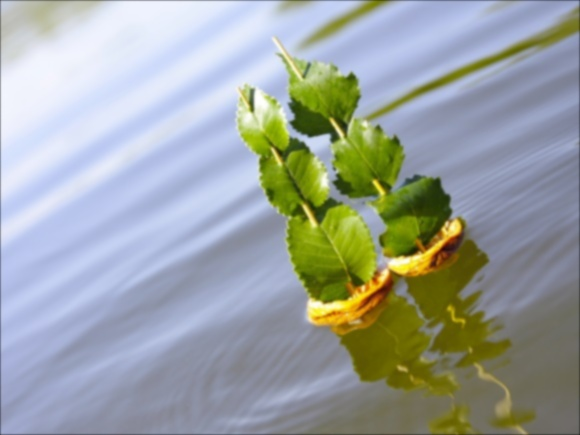
\includegraphics[width=0.23\linewidth]{./figures/2/lake-2-4.jpg} &
      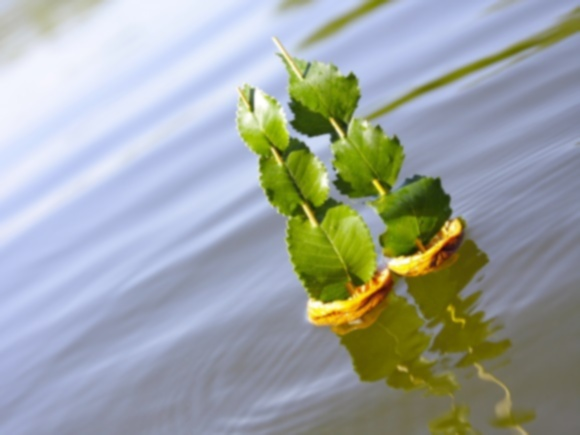
\includegraphics[width=0.23\linewidth]{./figures/2/lake-2-4-cv.jpg} \\
      a.~Original & b.~Our convolution & c.~OpenCV's convolution
      \end{tabular}
      \caption{Top row is the experiment number 2, which uses a $3 \times 3$ emboss filter. Bottom row is experiment number 4 which uses a $7 \times 7$ kernel to perform a gaussian blur.}
      \label{figure:conv}
    \end{figure*}

  \section{Color space reduction}

  \subsection{Color space reduction using only convolutions}
  At a first attempt to reduce color space, we used only convolutions. We have experimented with different kernel distributions with different kernel sizes:
  \begin{enumerate}
      \item Gaussian 7x7
      \item Gaussian 9x9
      \item Gaussian 15x15
      \item Gaussian 21x21
      \item Box Filter 3x3
      \item Box Filter 5x5
      \item Box Filter 9x9
      \item Box Filter 15x15
  \end{enumerate}

  The box filter has a kernel with all the weights containing the same values.
  In other words, this convolution calculates an average of the pixels in a NxN neighborhood for each pixel and then replaces
  the pixel value for that average in the original image. After applying this filter, the colors of neighbor pixels
  will be more similar as they are blended. The final result is a blurred image. Applying the box filter kernel of size 3 did not result
  in a much different image than the original. With a kernel of size 5, it was possible to notice a blur effect and the reduction of
  sharp edges or fine details in the image. With a kernel of size 9, an even more aggressive blur was applied to the image and
  depending on the resolution of the image, it was somewhat hard to interpret some parts of the image. Visually speaking, this seemed
  to be the best kernel size for a box filter. Finally, the box filter of size 15 resulted in images that
  had already lost too much information. All of the results can be seen in figure \ref{figure:color-reduction-box}.

  % Images with box filter applied (blur)
    \begin{figure*}[t]
      \centering
      \begin{tabular}{c c c c}
      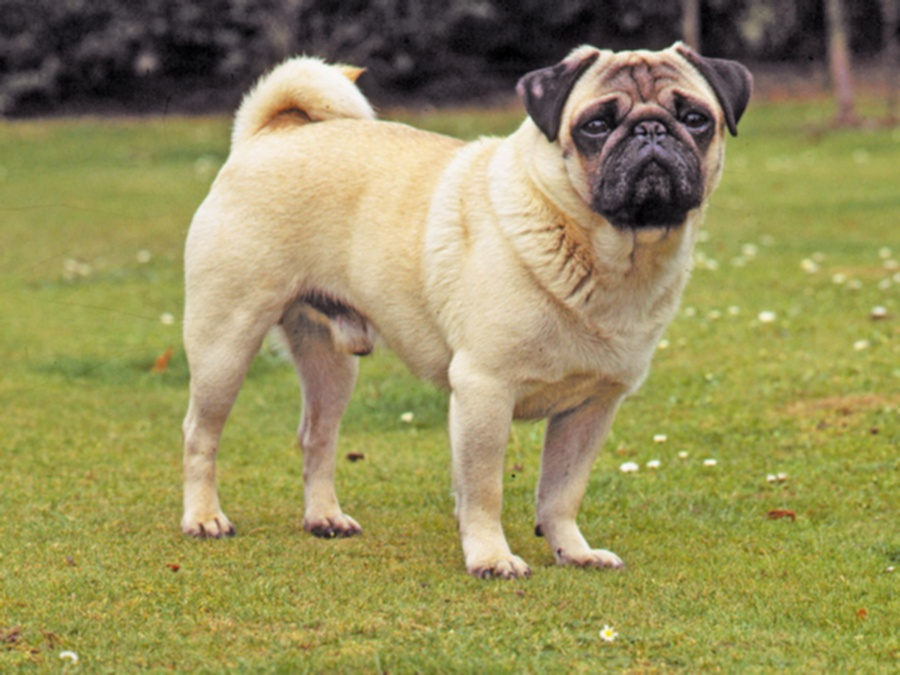
\includegraphics[width=0.22\textwidth]{./figures/3/dog-3-1-1-box3.jpg} &
      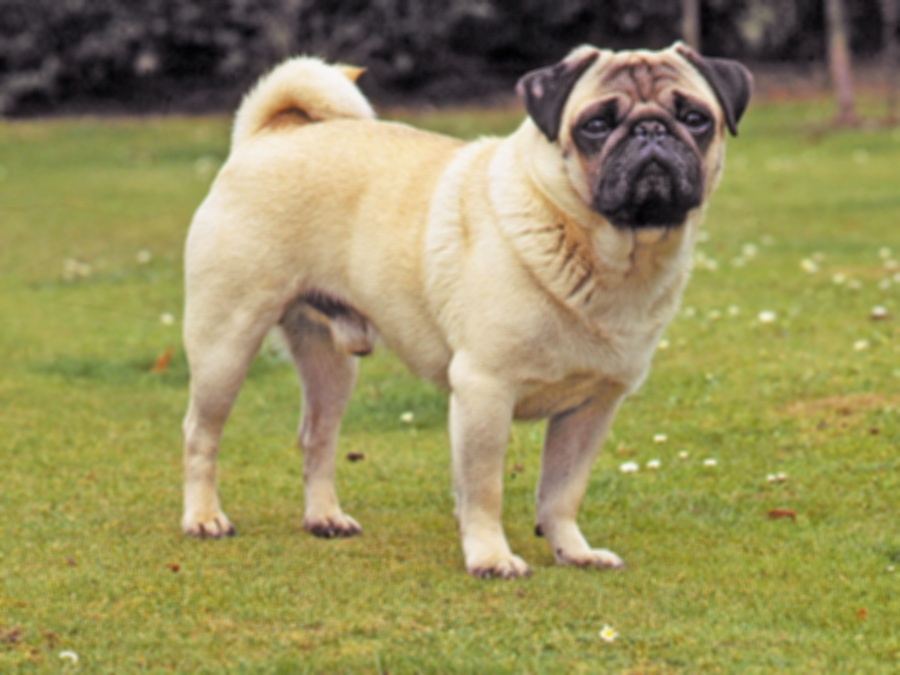
\includegraphics[width=0.22\textwidth]{./figures/3/dog-3-1-1-box5.jpg} &
      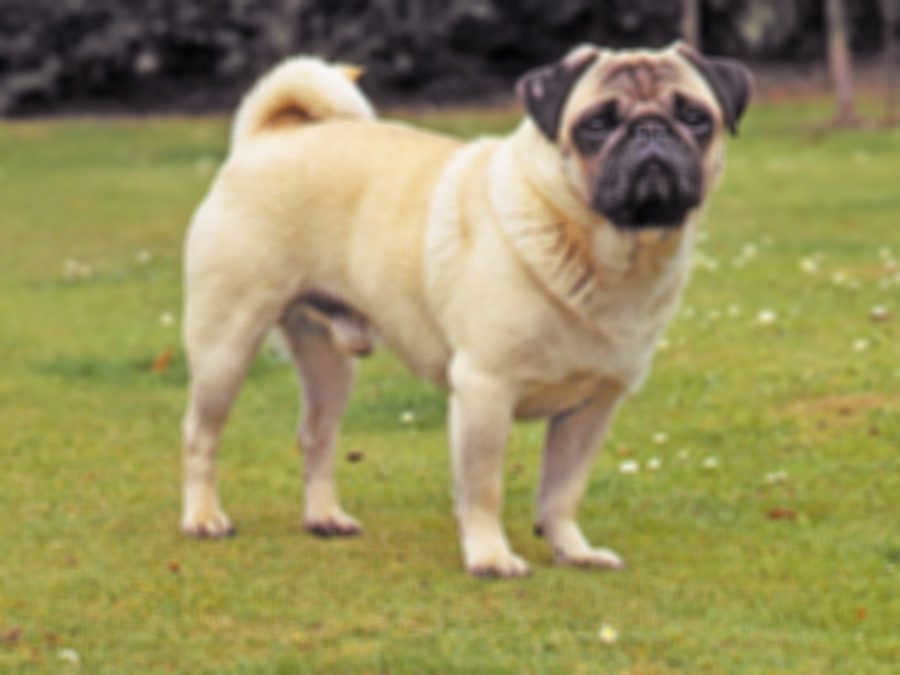
\includegraphics[width=0.22\textwidth]{./figures/3/dog-3-1-1-box9.jpg} &
      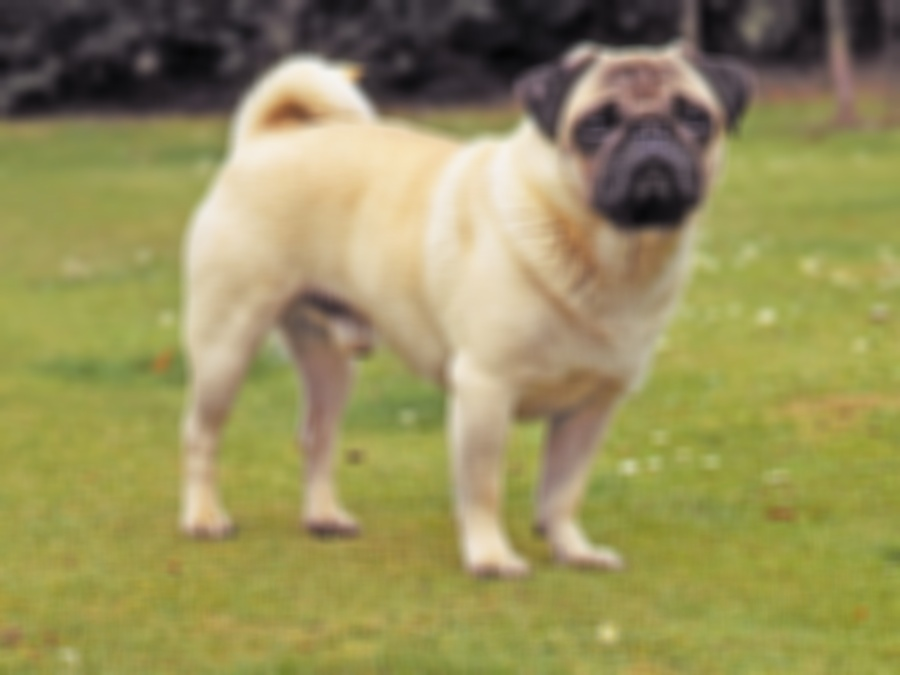
\includegraphics[width=0.22\textwidth]{./figures/3/dog-3-1-1-box15.jpg} \\
      a.~Kernel 3x3 & b.~Kernel 5x5 & c.~Kernel 9x9 & c.~Kernel 15x15
      \end{tabular}
      \caption{Color reduction using the box filter.}
      \label{figure:color-reduction-box}
    \end{figure*}

  The second convolution filter we tested was the gaussian filter.
  The goal of using this filter was the same as with the box filter: reduce the color difference between neighboring pixels.
  This would smooth fine details in textures, reduce noise and blend the colors of neighboring pixels.
  The main difference here was that instead of using a kernel with constant distribution (the box filter), we used
  a kernel with gaussian distribution.
  In order to have a visible effect on the image, we had to apply larger kernels than the ones used with the box filter.
  The larger the kernel size, the smoother the final image was.
  A difference from the box filter is that the gaussian filter kept more of
  original colors and there wasn't this effect of adding noise to the image.
  In a visual analysis, the best kernel size here was 15x15 as it had a significant impact on the final image but without
  blurring it too much in a way where we would lose important details of the original image.
  The results can be seen in figure \ref{figure:color-reduction-gaussian}.

% Images with gaussian filter applied (blur)
\begin{figure*}[t]
  \centering
  \begin{tabular}{c c c c}
  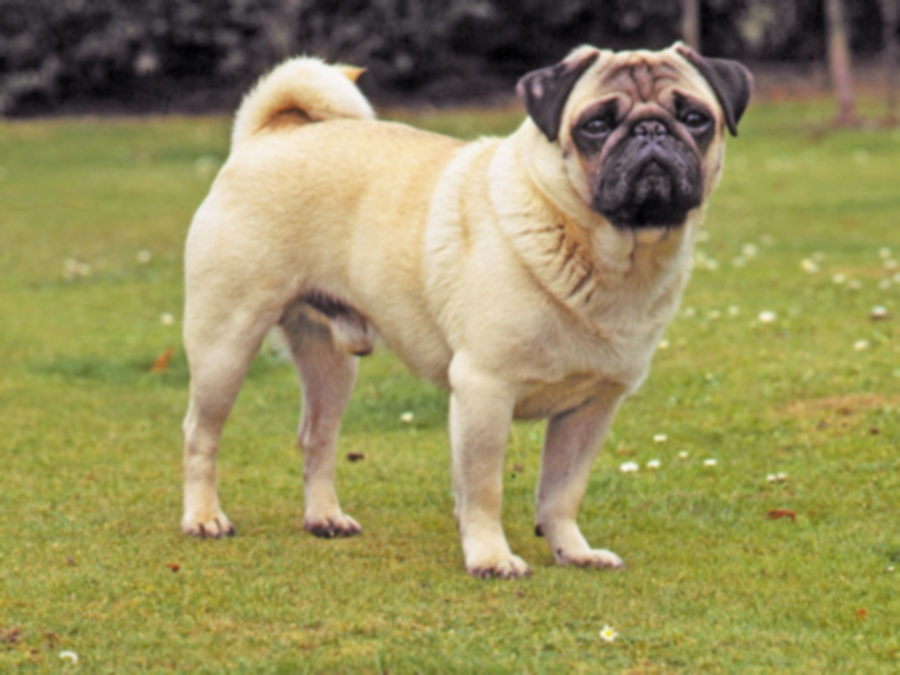
\includegraphics[width=0.22\textwidth]{./figures/3/dog-3-1-1-gaussian7.jpg} &
  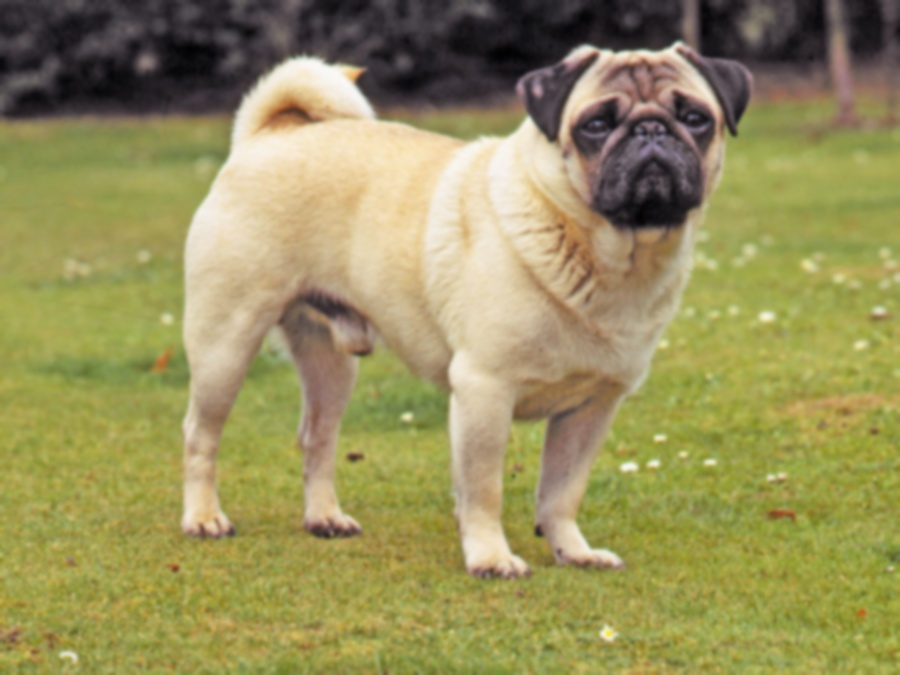
\includegraphics[width=0.22\textwidth]{./figures/3/dog-3-1-1-gaussian9.jpg} &
  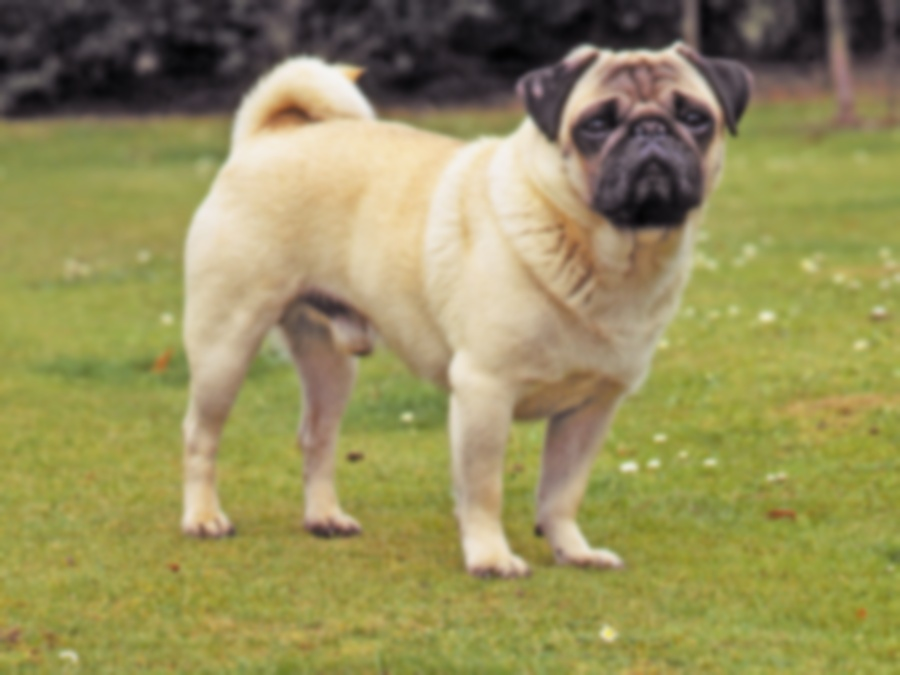
\includegraphics[width=0.22\textwidth]{./figures/3/dog-3-1-1-gaussian15.jpg} &
  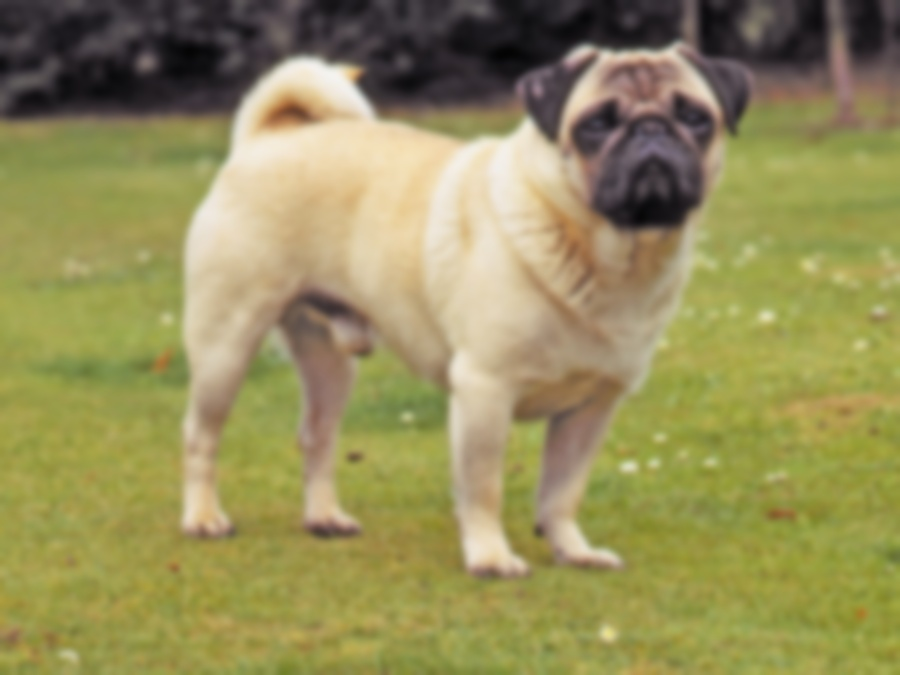
\includegraphics[width=0.22\textwidth]{./figures/3/dog-3-1-1-gaussian21.jpg} \\
  a.~Kernel 7x7 & b.~Kernel 9x9 & c.~Kernel 15x15 & c.~Kernel 21x21
  \end{tabular}
  \caption{Color reduction using the gaussian filter.}
  \label{figure:color-reduction-gaussian}
\end{figure*}

  Besides doing a visual analysis, we plotted the color histograms as an attempt to verify or validate
  the effectiveness of the filters used. We used two different types of histograms:
  the RGB histogram and the HSV histogram. The first one shows the distribution of pixels for channels
  R(ed), G(reen) and B(lue) while the second one shows the distribution of pixels in the space H(ue) and S(aturation).
  We ignored the V (brightness) for the sake of simplicity and assumed that the H and S dimensions would be significant
  enough to analyze the color distribution in the image.

  First, let's look at the RGB histograms in figure \ref{figure:dog-rgb-hist}.
  There is a subtle difference between the distribution in the original
  image and the filtered ones. The distribution seems to get more concentrated on those 2 peaks after the filtering
  (i.e. those two curves seem to get narrower).
  However, it's not quite clear what is the relationship between these histograms and
  what we see in \ref{figure:color-reduction-gaussian} or \ref{figure:color-reduction-box}.
  If we look at figure \ref{figure:lake-rgb-hist}, it seems that a high concentration of blue points (close to zero)
  ended up being distributed to other parts of the histogram. Nevertheless, this phenomenon seemed very
  particular of this image as for the other images tested in our dataset, it was very hard to translate the changes
  in the RGB histogram to a sense of how effective the each applied filter was.

  Regarding the HSV histograms \cite{b7}, applying the convolutions on the original image seemed
  to approximate points to a denser region of the HS space. In \ref{figure:dog-hsv-hist}(a),
  the distribution of points is more sparse whereas in \ref{figure:dog-hsv-hist}(b) and \ref{figure:dog-hsv-hist}(c)
  the points seem to be more concentrated.
  On the other hand, looking at the figure \ref{figure:lake-hsv-hist}, there is barely any difference between the 3 histograms.

  Overall, looking at the color histograms (either HSV or RGB) does not seem like an effective method to
  measure or verify how good or bad the selected filters are for this cartoonization application.


  % Dog: histograms RGB
  \begin{figure*}[t]
  \centering
  \begin{tabular}{c c c}
  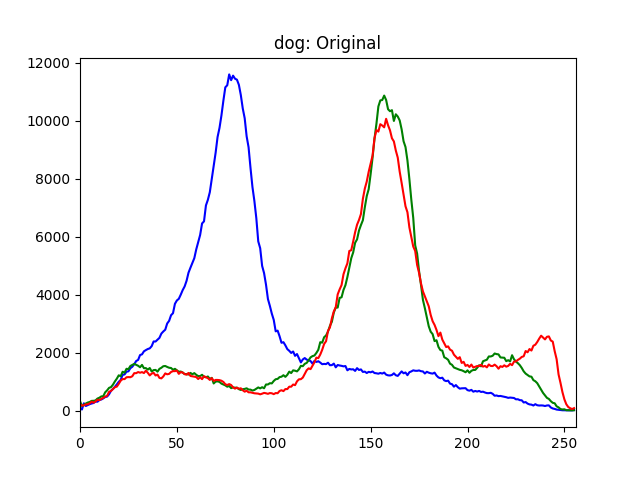
\includegraphics[width=0.3\textwidth]{./figures/3/dog-rgbhist.png} &
  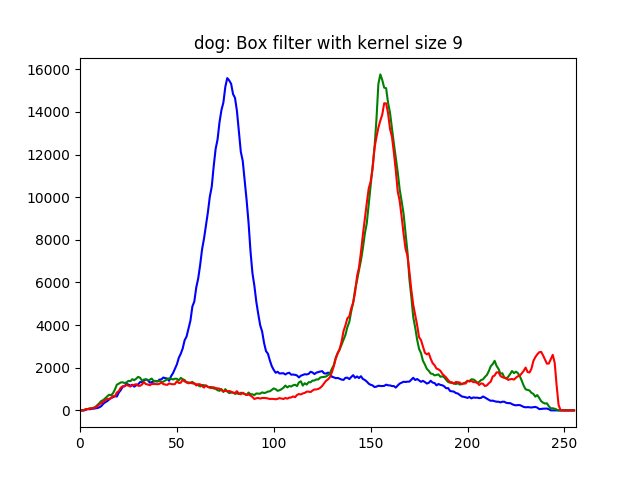
\includegraphics[width=0.3\textwidth]{./figures/3/dog-3-1-1-box9-rgbhist.png} &
  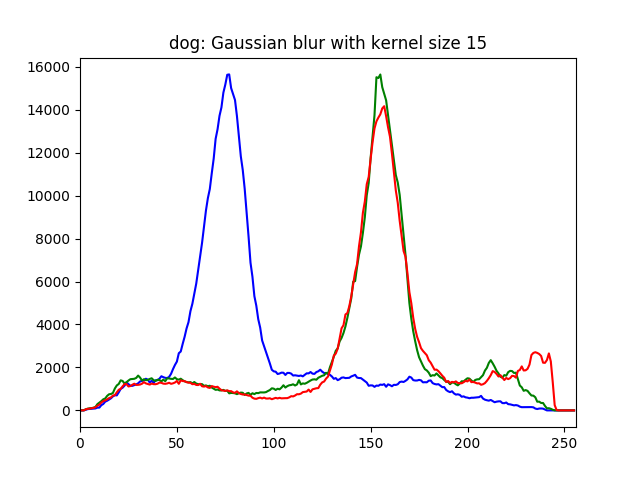
\includegraphics[width=0.3\textwidth]{./figures/3/dog-3-1-1-gaussian15-rgbhist.png} \\
  a.~Original & b.~After Box Filter & c.~After Gaussian Filter
  \end{tabular}
  \caption{Dog image: Comparison of histograms.}
  \label{figure:dog-rgb-hist}
\end{figure*}

  % Lake: histograms RGB
  \begin{figure*}[t]
  \centering
  \begin{tabular}{c c c}
  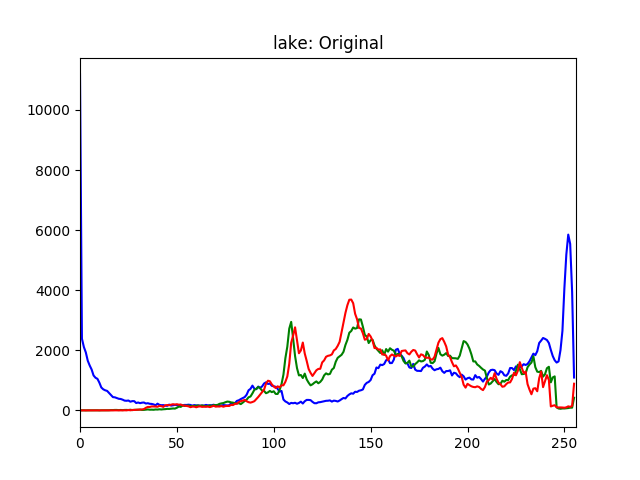
\includegraphics[width=0.3\textwidth]{./figures/3/lake-rgbhist.png} &
  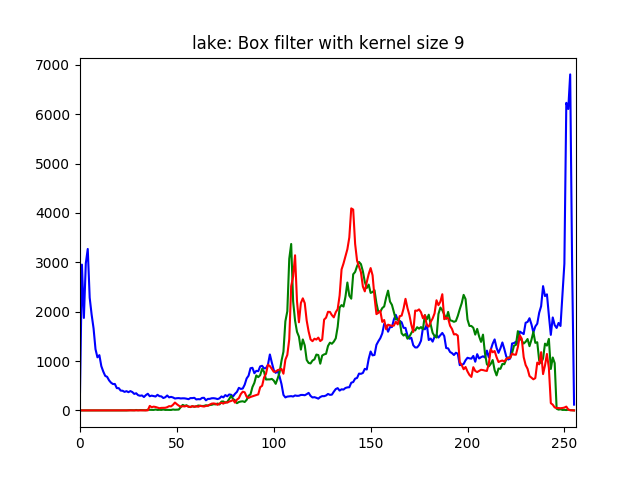
\includegraphics[width=0.3\textwidth]{./figures/3/lake-3-1-1-box9-rgbhist.png} &
  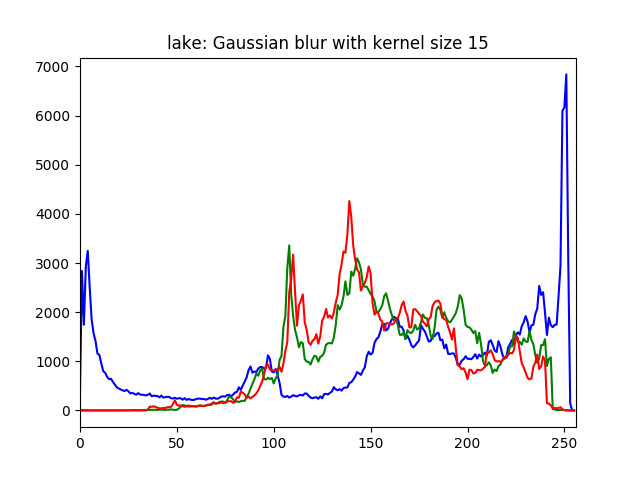
\includegraphics[width=0.3\textwidth]{./figures/3/lake-3-1-1-gaussian15-rgbhist.png} \\
  a.~Original & b.~After Box Filter & c.~After Gaussian Filter
  \end{tabular}
  \caption{Lake image: Comparison of histograms.}
  \label{figure:lake-rgb-hist}
  \end{figure*}

 % Dog: histograms HSV
  \begin{figure*}[t]
  \centering
  \begin{tabular}{c c c}
  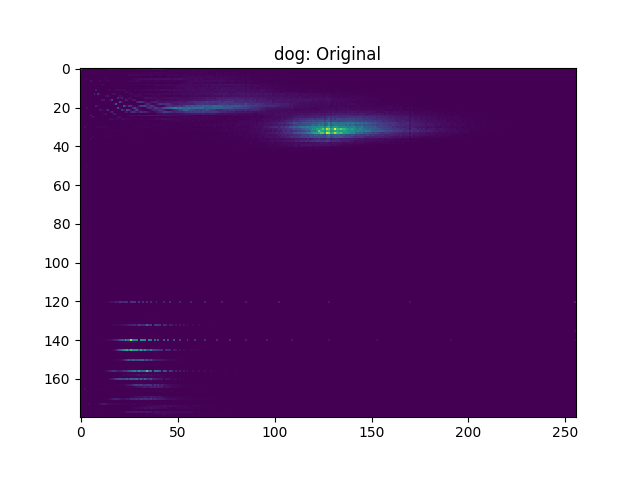
\includegraphics[width=0.3\textwidth]{./figures/3/dog-hsvhist.png} &
  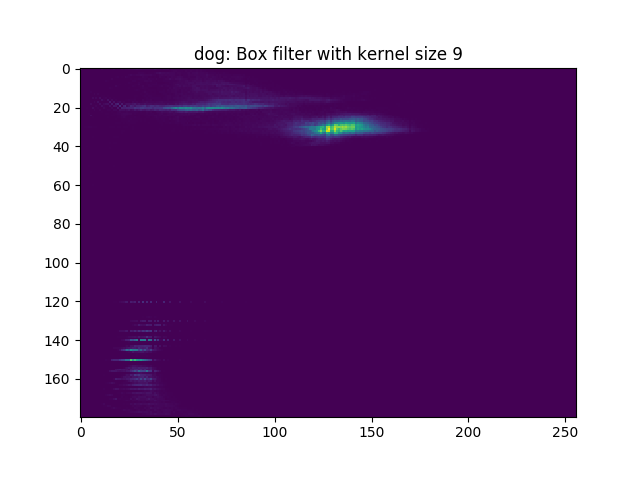
\includegraphics[width=0.3\textwidth]{./figures/3/dog-3-1-1-box9-hsvhist.png} &
  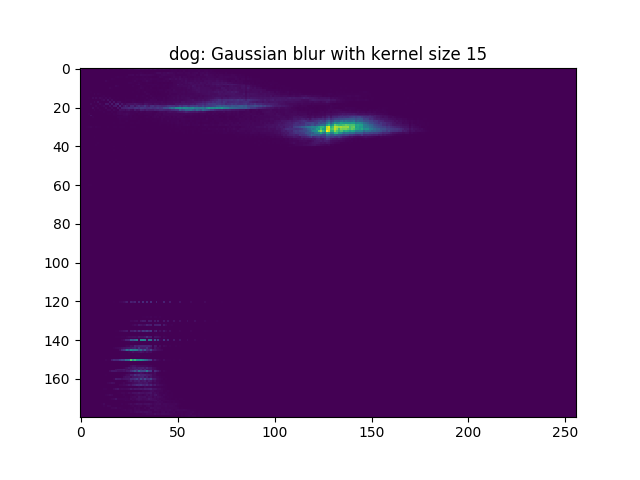
\includegraphics[width=0.3\textwidth]{./figures/3/dog-3-1-1-gaussian15-hsvhist.png} \\
  a.~Original & b.~After Box Filter & c.~After Gaussian Filter
  \end{tabular}
  \caption{Dog image: Comparison of histograms.}
  \label{figure:dog-hsv-hist}
  \end{figure*}

   % Lake: histograms HSV
  \begin{figure*}[t]
  \centering
  \begin{tabular}{c c c}
  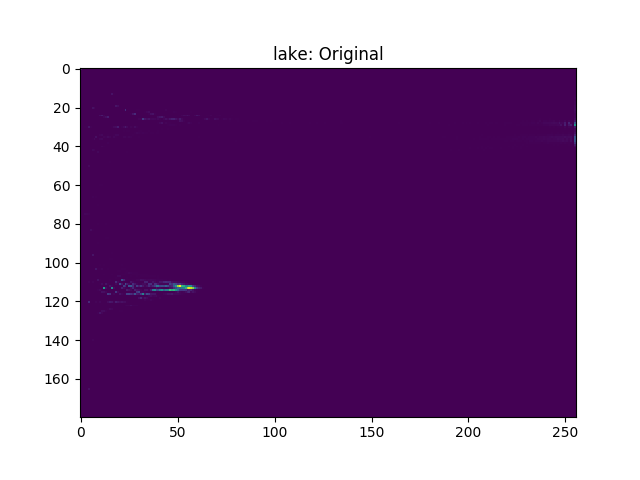
\includegraphics[width=0.3\textwidth]{./figures/3/lake-hsvhist.png} &
  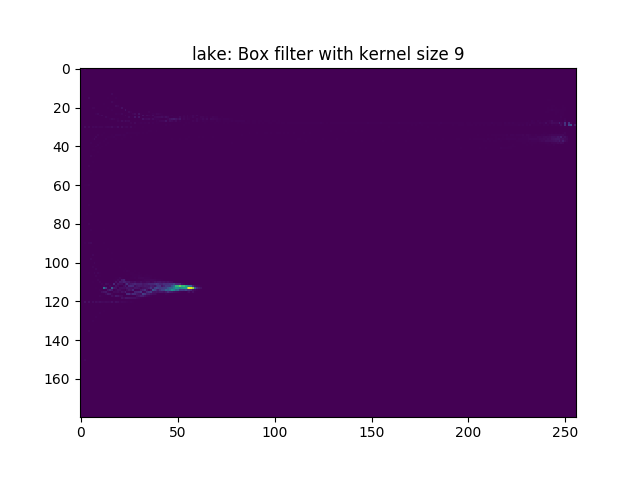
\includegraphics[width=0.3\textwidth]{./figures/3/lake-3-1-1-box9-hsvhist.png} &
  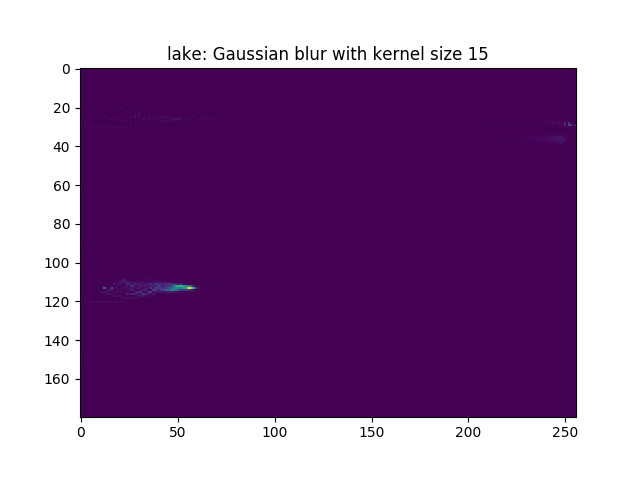
\includegraphics[width=0.3\textwidth]{./figures/3/lake-3-1-1-gaussian15-hsvhist.png} \\
  a.~Original & b.~After Box Filter & c.~After Gaussian Filter
  \end{tabular}
  \caption{Lake image: Comparison of histograms.}
  \label{figure:lake-hsv-hist}
  \end{figure*}


  After all of the experiments we have run trying to reduce color space,
  we are fairly certain that using only convolutions is not enough for a final polished cartoonish effect.
  Cartoons have a limited number of colors and for that, we need a color quantization step which
  cannot be achieved only through convolutions. Nevertheless, this is an important part of the pipeline to cartoonize
  images as it reduces image noise, reduces the complexities and details of textures
  and transforms the image into a more homogeneous set of colors.

    % [edgar] Reviewed till here

  \subsection{Color space reduction using clusterization}
  Trying to improve on the results obtained by using only convolution, we use
  clusterization to reduce the color space. The approach adopted uses the
  implementation of k-means provided by OpenCV, with $k$ being the number of
  colors of the resulting image. The algorithm works as follows\cite{b6}:

  \begin{enumerate}
      \item Algorithm randomly chooses $k$ centroids.
      \item Then, for each pixel, it calculates the distance from the pixel to
          all centroids. The pixel is assigned to the cluster of the closer
          centroid.
      \item Then, for each cluster, it calculates the average position of the pixels in
          the cluster. This average will be the new centroid of the cluster.
      \item Repeats the steps 2 and 3 until all the centroids converge to fixed
          points or the stop criteria is satisfied.
  \end{enumerate}

  In order to get better results from clusterization, we execute it after a
  median blur filter, used to blur the image. The blurred image has less noise
  and less high-frequency elements (i.e. one pixel will not be as much different
  from its neighbors), so that the resulting clusters will be larger and the
  image will be closer to what a cartoon looks like.

  The relevant code snippet is presented below:

  \lstinputlisting[caption={Clusterization with k-means},
  firstline=43, lastline=57]{../src/cartoonize.py}

  First, the input image $img$ is blurred using a median blur filter, then the
  resulting output from the blurring process becomes the input for the
  clusterization procedure. In this phase, the image is first reshaped to 2
  dimensions, then the clusterization is performed. In this case,
  $NUMBER\_OF\_COLORS = 16$. Then, using the centers of the clusters, we
  construct the output image, with 16 colors.

  \begin{figure*}[t]
    \centering
    \begin{tabular}{c c}
    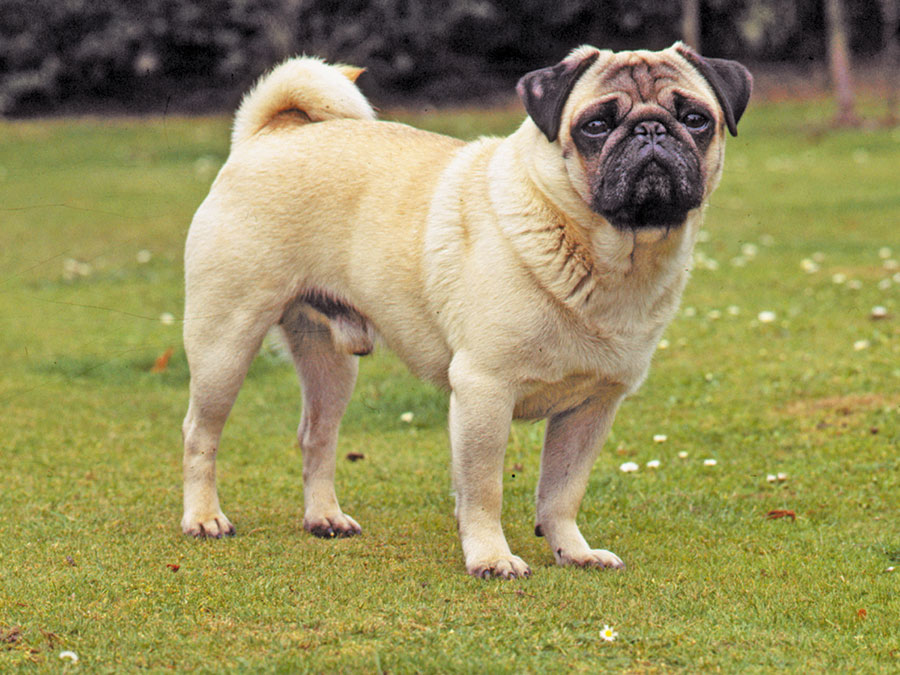
\includegraphics[width=0.35\textwidth]{./figures/3/dog.jpg} &
    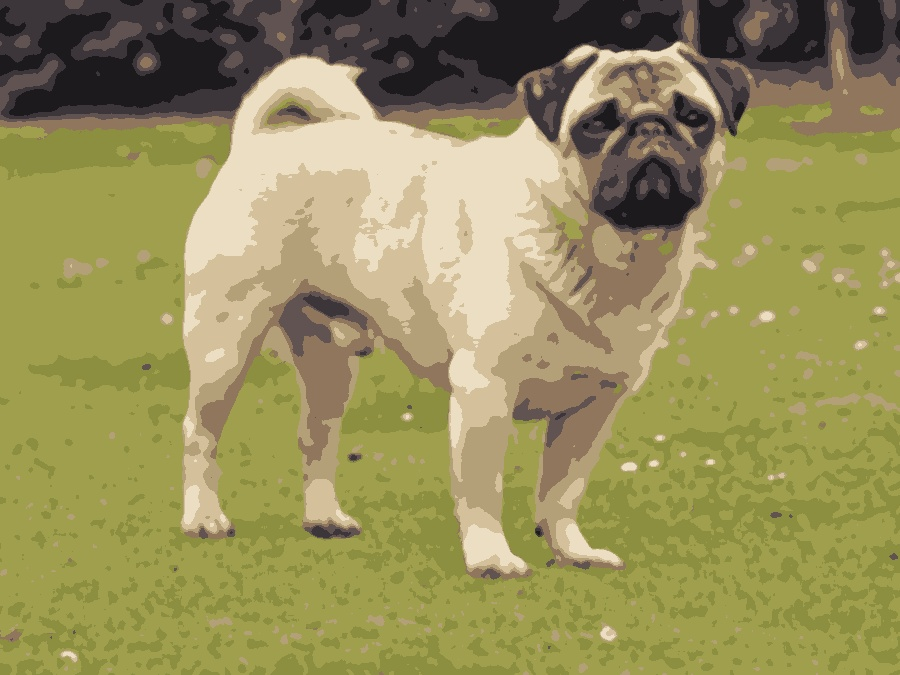
\includegraphics[width=0.35\textwidth]{./figures/3/dog-3-1-2.jpg} \\
    a.~Original image & b.~Color-reduced image
    \end{tabular}
    \caption{Comparison between an image and the result of the color reduction
    process.}
    \label{figure:colorreduction}
  \end{figure*}

  Figure~\ref{figure:colorreduction} shows the result of this process for an
  image of a dog. We can see clearly that there are way fewer colors and fewer
  details in the resulting image, which are characteristics of cartoons.

  \begin{figure*}[t]
    \centering
    \begin{tabular}{c c}
    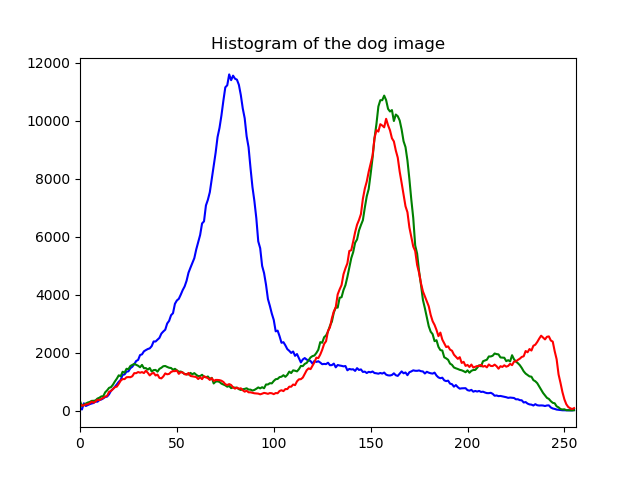
\includegraphics[width=0.35\textwidth]{./figures/3/dog-3-1-2-hist.png} &
    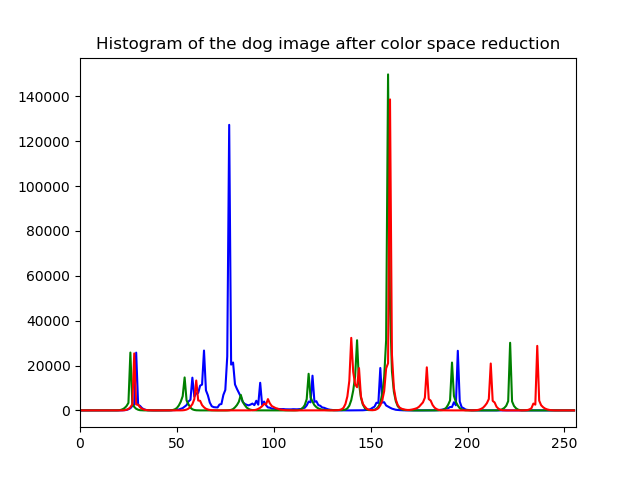
\includegraphics[width=0.35\textwidth]{./figures/3/dog-3-1-2-color-hist.png} \\
    a.~Histogram for the original image & b.~Histogram for the color-reduced image
    \end{tabular}
    \caption{Comparison between the histograms of the input image and the image
    result of the color reduction process.}
    \label{figure:colorreductionhist}
  \end{figure*}

  In figure~\ref{figure:colorreductionhist}, we can see the histogram of the
  original image (left) and the histogram of the output image of the color
  space reduction process (right). The histogram of the resulting image looks
  discretized, with some spikes on some color intensities and zero on the other
  intensities, which makes sense because now we have less different colors to
  ``distribute'' to the pixels.

  \section{Edge detection}
  Edge detection refers to the process of identifying and locating sharp discontinuities in an image. The discontinuities are abrupt changes in pixel intensity which characterize boundaries of objects in a scene\cite{b4}. There are many ways to perform edge detection, we did experiments using predefined kernels, thus performing the convolution, and the algorithm known as Canny Edge Detection\cite{b5}.
  
  \subsection{Edge detection using convolution}
  We selected 9 different kernels: Sobel operator (both directions), Robert's cross operator (both directions), Prewitt's operator (both directions), two discrete approximations to the Laplacian filter and a precomputed Laplacian of Gaussian kernel. We tested each kernel in three different test images and we selected those which gave the best result for each image. Figure \ref{figure:edge1} shows the convolved images, their originals can be found in Figure \ref{figure:conv}. The choice of which results to show was easy for some kernels, which had darken the images, and difficult for others, because the result were very similar, but we chose based on the details and how the filters managed to separate some important aspects of the image, like body, face, lamps, etc.
  
  As analyzed by Maini et. al.\cite{b4}, Sobel, Robert's cross and Prewitt's are simple to implement, once you know the kernels you perform the convolution, they also detect edges and their orientation. Unfortunately, they are very sensitive to noise and highly inaccurate. The two discrete Laplace approximation filters, or second directional derivative, detect edges and their orientations, have fixed characteristics in all directions, but respond to some of the existing edges and are also sensitive to noise.
  The Laplacian of Gaussian (LoG) finds the correct places of edges and tests wider area around the pixel. However, this filter does not work well at the corners, curves nor where the gray level intensity function varies. Moreover, we can not find the orientation of edge due to the use of the Laplacian filter.
  
  \subsection{Edge detection using Canny Edge Detection}
  In his paper, Canny followed a list of criteria to improve methods of edge detection in his time. The first is the low error rate. It is important that edges occurring in images should not be missed and that there be no responses to non-edges. The second criterion is that the edge points be well localized. That is, the distance between the edge pixels as found by the detector and the actual edge is to be at a minimum. A third criterion is to have only one response to a single edge\cite{b4}.
  
  In order to implement the Canny edge detector algorithm, a series of steps must be followed.
  \begin{enumerate}
      \item The first step is to compute gradient directions.
      \item Then for each pixel, compute smoothed 1$D$ directional derivative in the gradient direction. 
      \item Find the maximum magnitude of these derivatives.
      \item Performs the synthesis of edgels obtained for different smoothing
  \end{enumerate}
  
  Canny Edge Detection improves signal to noise ratio and has better detection specially in noise conditions, but has complex computations, false zero crossing, and is more time consuming\cite{b4}. Figure \ref{figure:edge2} shows the result of performing Canny Edge Detection in the same images as in Figure \ref{figure:conv}.
  
    \begin{figure*}[tb]
      \centering
      \begin{tabular}{c c}
      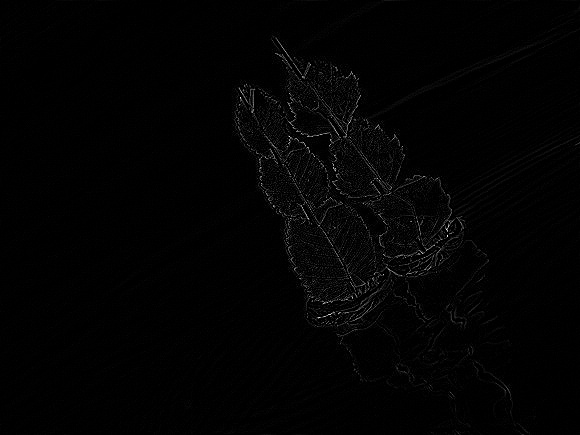
\includegraphics[width=0.35\linewidth]{./figures/3/lake-3-2-1-1.jpg} &
      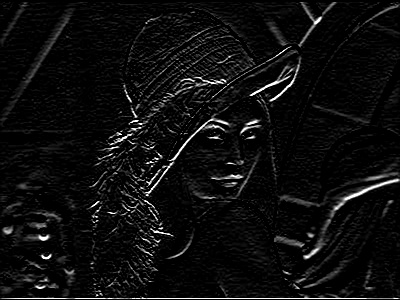
\includegraphics[width=0.35\linewidth]{./figures/3/lena-3-2-1-2.jpg} \\
      a.~Laplacian of Gaussian centered on zero & b.~Sobel in Y
      \end{tabular}
      \caption{Extracting edges using convolution operation and different kernels}
      \label{figure:edge1}
    \end{figure*}
  
  \begin{figure*}[tb]
      \centering
      \begin{tabular}{c c}
      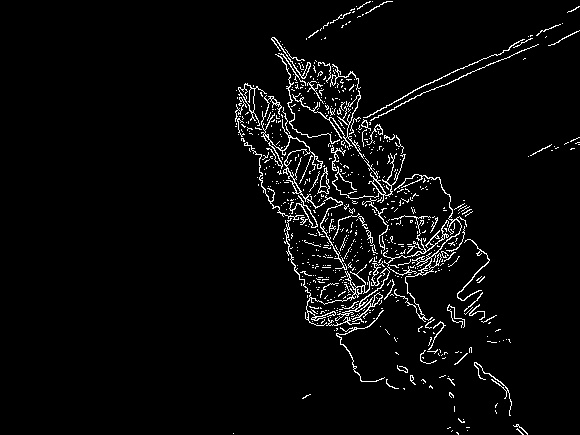
\includegraphics[width=0.35\linewidth]{./figures/3/lake-3-2-1-1-canny.jpg} &
      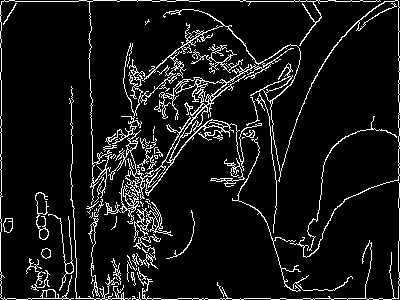
\includegraphics[width=0.35\linewidth]{./figures/3/lena-3-2-1-2-canny.jpg} \\
      a.~Canny with min, max & b.~Canny with min, max\\
      ~thresholds of 100 and 100 & ~thresholds of 50 and 300\\
      \end{tabular}
      \caption{Extracting edges using Canny edge detector algorithm}
      \label{figure:edge2}
    \end{figure*}
  
  \section{Line drawing and Cartoonization pipeline}
  % Once you have detected edges from the image, you may want to binarize the edge image (if necessary) and render it on top of the color-reduced image in black color.

    % Show the final images using both methods for color reduction and edge detection. Are the results significantly different? Which combinations are better and why do you think so? What if you, instead of detecting edges from the original image, detect edges from the color-reduced ones? Does it improve something?
    % Real-world images contain very complex shapes and textures, and edge detection algorithms may end up with noise, by highlighting undesirable edges. Since a cartoon is way less complex, your final images may not be so convincing still. On the other side, you can end up with relevant edges being too thin for a cartoon.
    %So make a final effort and look for a way to improve those borders. The first thing you may think about is mathematical morphology, but feel free to explore better (still simple) alternatives. Remember always to keep your code simple.
    %Describe your approach and show your results. Analyze its impact on the performance of your method.
    %You can provide a few code snippets to better illustrate your ideas.

    After running some experiments with edge detection algorithms, we binarized the edge images to create borders
    for the cartoonized image. Here is a summary of all the variations we have tried for the cartoonization pipeline:

    \begin{table}[h]
    \centering
        \begin{tabular}{|c c c c c|}
        \hline
            Variation & Colored/BW & Edge & Reduced/Original & Border\\
            \hline\hline
            1 & Colored & LoG & Reduced & None\\
            \hline
            2 & Colored & Canny & Reduced & None\\
            \hline
            3 & Colored & Canny & Original & None\\
            \hline
            4 & BW & Canny & Original & None\\
            \hline
            5 & BW & Canny & Original & Closed\\
            \hline
            6 & -- & -- & -- & --\\
            \hline
            7 & BW & Canny & Original & Dilated\\
            \hline
            8 & BW & Canny & Reduced & Dilated\\
        \hline
        \end{tabular}
        \vspace{1pt}
        \caption{Variations of the cartoonization pipeline.}
        \label{table:variations}
        \vspace{-5pt}
    \end{table}

    Table \ref{table:variations} shows the different combinations of the following variations
    \begin{itemize}
    \item Colored/BW: either using a colored or black and white image as an input to the edge detection algorithm
    \item Edge algorithm: LoG (Laplacian of Gaussian) or Canny
    \item Reduced/Original: either using the color reduced image or the original image as an input to the edge detection algorithm
    \item Border: we have tried the morphological operator of close and dilate to improve the border rendering
    \end{itemize}

    This report only includes the best results which came from variations 4 (see figure \ref{figure:cartoonized-var4})
    and 8 (see figure \ref{figure:cartonized-var8}).
    All of the variations can be downloaded from our gitlab CI pipeline as artifacts of the ``cartoonization'' test.

    \begin{figure*}[h]
      \centering
      \begin{tabular}{c c}
      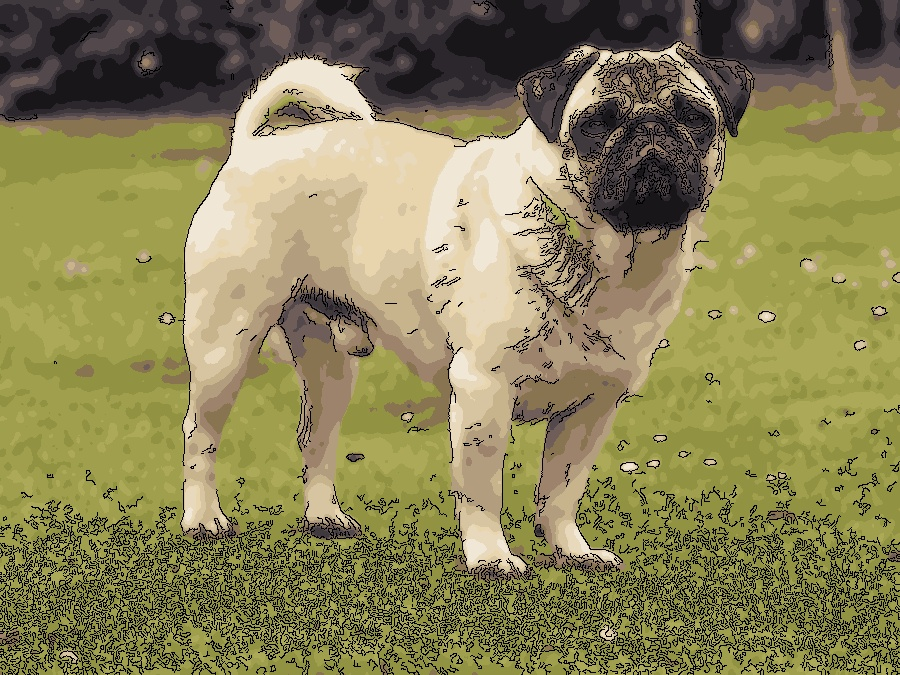
\includegraphics[width=0.35\linewidth]{./figures/cartoonize/dog-3-2-2-var4.jpg} &
      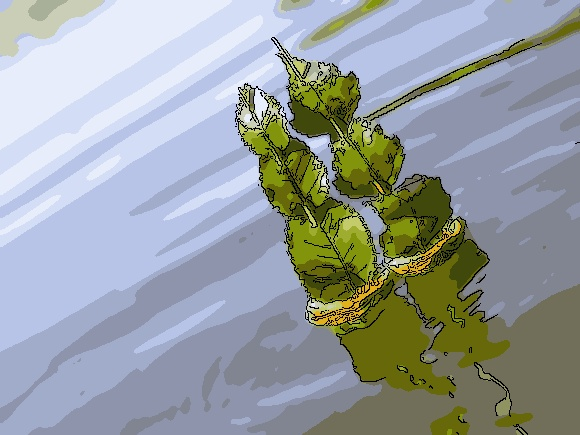
\includegraphics[width=0.35\linewidth]{./figures/cartoonize/lake-3-2-2-var4.jpg} \\
      a. Dog & b. Lake \\
      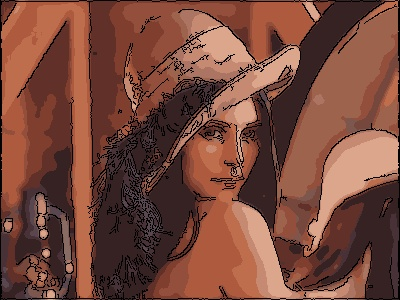
\includegraphics[width=0.35\linewidth]{./figures/cartoonize/lena-3-2-2-var4.jpg} &
      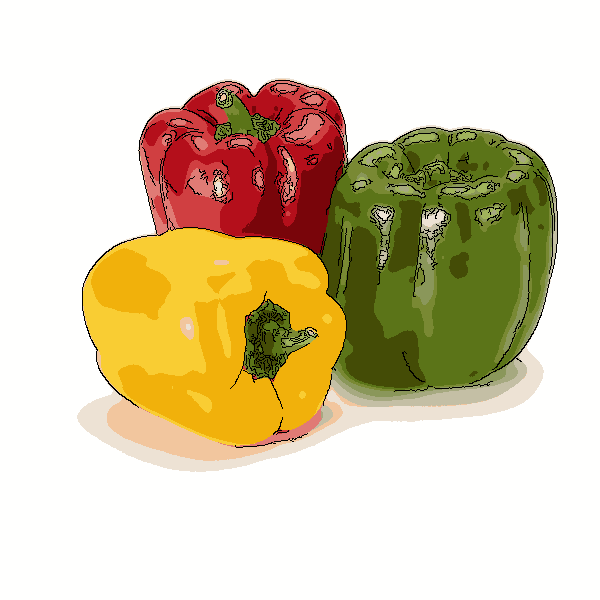
\includegraphics[width=0.35\linewidth]{./figures/cartoonize/peppers-3-2-2-var4.png} \\
      c. Lena & d. Peppers \\
      \end{tabular}
      \caption{Cartoonization: variation 4}
      \label{figure:cartoonized-var4}
    \end{figure*}

    \begin{figure*}[h]
      \centering
      \begin{tabular}{c c}
      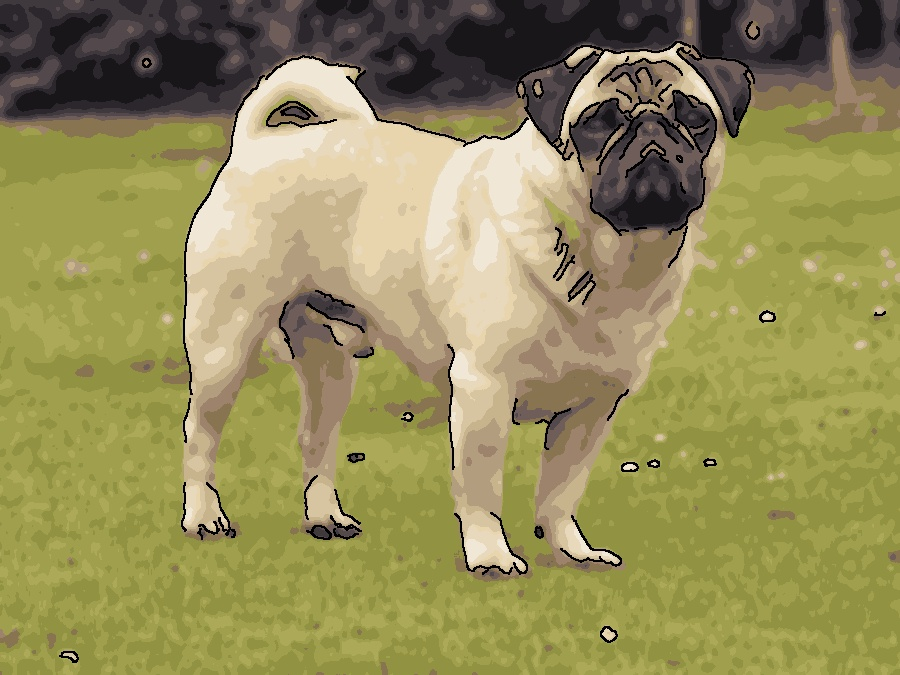
\includegraphics[width=0.35\linewidth]{./figures/cartoonize/dog-3-2-2-var8.jpg} &
      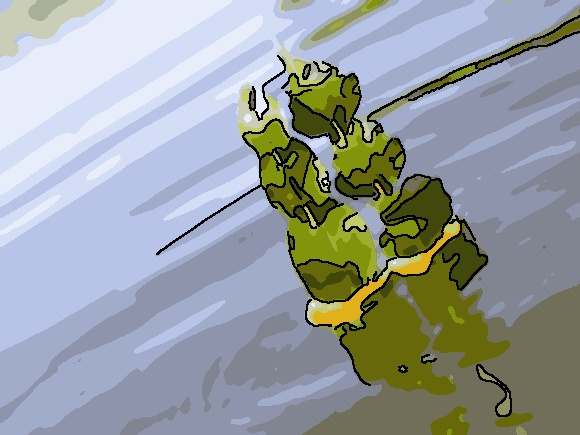
\includegraphics[width=0.35\linewidth]{./figures/cartoonize/lake-3-2-2-var8.jpg} \\
      a. Dog & b. Lake \\
      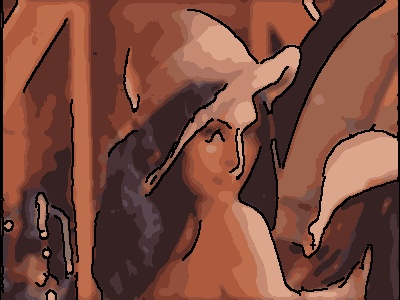
\includegraphics[width=0.35\linewidth]{./figures/cartoonize/lena-3-2-2-var8.jpg} &
      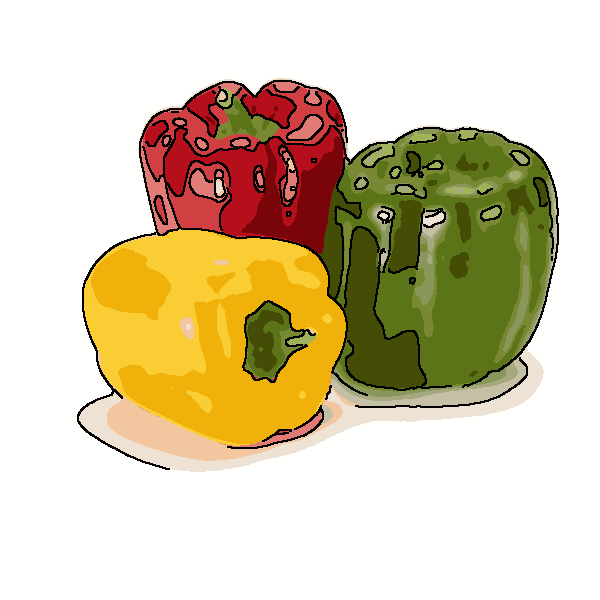
\includegraphics[width=0.35\linewidth]{./figures/cartoonize/peppers-3-2-2-var8.png} \\
      c. Lena & d. Peppers \\
      \end{tabular}
      \caption{Cartoonization: variation 8}
      \label{figure:cartonized-var8}
    \end{figure*}

    Binarizing the edge images was not an easy task as we were manually setting the thresholds that worked best.
    Well suited thresholds for detecting edges in one image were not necessarily successful in others.
    Especially for our dataset where we picked 4 very distinctive images.
    We have experimented with an adaptive threshold function in variation 1 but the results were far from successful -
    edges were detected all over the image.

    We would like now to analyze two most successful variations.
    Let's start with variation 4 which is very simple.
    It reads the original image as black and white and then applies the Canny edge detector with fixed and manually set thresholds.
    Although the edges are not all desired, this very simple initial attempt was able to produce some interesting
    cartoonized images. In figure \ref{figure:cartoonized-var4}, you can see how the Dog (a)
    image has detected lots of edges in the grass which were not desired.
    These same undesired edges can be seen in the leaves of the Lake (b) image and in the hair of the Lena (c) image.
    This variation lacked a very important step which is the application of a gaussian filter before running the edge detection algorithm.
    Without this low-pass filter to smooth the image, any noise or small details in the image will be taken as edges.

    In variation 8 though, we did apply a gaussian filter on top of the color reduced image converted to black and white.
    We noticed that this is an important step in order to reduce those false edges which appear
    in small details of the image (as noted in variation 4). Once the gaussian filter smoothed the image,
    then we apply the Canny edge detector. As you can see in figure~\ref{figure:cartonized-var8},
    we were able to reduce the number of edges while still maintaining the ones that divide the different
    colors of our cartoon.
    This doesn't seem like a perfect result though as the Lena (c) image doesn't have well-defined edges in the face region.
    Moreover, the edges in the Dog (a) image has some discontinuities.
    As future work, one could try to use adaptive algorithms to set the thresholds of the Canny edge detector.

    We also worked on improving the borders which were too thin for a cartoon.
    Basically, we tested two different morphological operators: closing and dilation.
    The close morphological operator should be able to fill any gaps or dents in the borders
    in order to have borders with constant width.
    However, as the edge detectors in this variation captured too many edges,
    the morphological operator only highlighted those undesired edges.
    The best results we obtained were with variation 8 (see figure \ref{figure:cartonized-var8})
    where the edges found were clean and we only enhanced them by applying the dilation morphological operator.
    This operator increases the width of the border.

  \section{Conclusion}
    The objective of this work was to create cartoonized images from real photograph images.
    This process was broken down into three major steps: color reduction, edge detection and border rendering.
    For color reduction, we concluded that convolutions were an important step, although not sufficient for a
    convincible cartoonized effect. Applying a median filter and using the k-means algorithm to quantize the colors
    of the image allowed us to achieve smooth homogeneous surfaces with a reduced color pallette. For the edge detection,
    the Canny algorithm produced the best results when compared to other methods based on convolution.
    As for the border rendering, we were able to create thicker borders - typically seen in cartoons - with the morphological operator of dilation.

\begin{thebibliography}{00}
    \bibitem{b1} Goodfellow, I., Bengio, Y., Courville, A., \& Bengio, Y. (2016). ``Deep learning'' (Vol. 1). Cambridge: MIT press.
    \bibitem{b2} Kazemi, H. (2017, February 6). Image Filtering [Web log post]. Retrieved August 22, 2018, from http://machinelearninguru.com/
    \bibitem{b3} Szeliski, R. (2010). Computer vision: algorithms and applications. Springer Science \& Business Media.
    \bibitem{b4} Maini, R., \& Aggarwal, H. (2009). Study and comparison of various image edge detection techniques. International journal of image processing (IJIP), 3(1), 1-11.
    \bibitem{b5} Canny, J. F. (1983). Finding edges and lines in images.
    \bibitem{b6} Understanding K-Means Clustering [Web log post]. Retrieved
        September 1, 2018, from
        \url{https://docs.opencv.org/3.4.2/de/d4d/tutorial\_py\_kmeans\_understanding.html}
    \bibitem{b7}
        Histograms - 3 : 2D Histograms. Retrieved on September 7, 2018, from
        \url{https://docs.opencv.org/3.1.0/dd/d0d/tutorial_py_2d_histogram.html}
    \bibitem{b8}
        Histograms - 1 : Find, Plot, Analyze !!!. Retrieved on September 7, 2018, from
        \url{https://docs.opencv.org/3.1.0/d1/db7/tutorial_py_histogram_begins.html}
\end{thebibliography}
\end{document}

% TODO: [edgar] I want to add some other histograms as an appendix
% TODO: [edgar] need to put H and S in the HSV histograms for the axis